%========================================================================
% NIP'AJIN Autorenpaket v1.1, (C) Markus Leupold-Löwenthal
%========================================================================
% Dieses Werk untersteht folgender Lizenz:
% Namensnennung–Weitergabe unter gleichen Bedingungen 3.0 Österreich
% (CC BY-SA 3.0) http://creativecommons.org/licenses/by-sa/3.0/at/
%========================================================================

\documentclass{article}

\usepackage{nipajin}

\hyphenation{Blatt-hälfte}

% --- Hyperlinks und PDF ----------------------------------------------------
\hypersetup{
	pdftitle={NIP'AJIN},
	pdfauthor={Max Musterperson},
	pdfsubject={Ein Szenario für das leichtgewichtiges, freie Rollenspielsystem	NIP'AJIN}, 
	pdfkeywords={nipajin, nip'ajin, Rollenspiel, System, frei, RSP, RPG}
}

% ###########################################################################
% ###########################################################################
% ###########################################################################
% ###########################################################################
% ###########################################################################

\begin{document}\fftext

% ### COVER #################################################################

\renewcommand{\hintergrund}{images/cover.jpg}
% Special Relativity
\thispagestyle{empty}
\raisebox{0mm}[0mm][0mm]{%
\parbox{8.5in}{
\vspace*{236mm}\hspace{-38.5mm}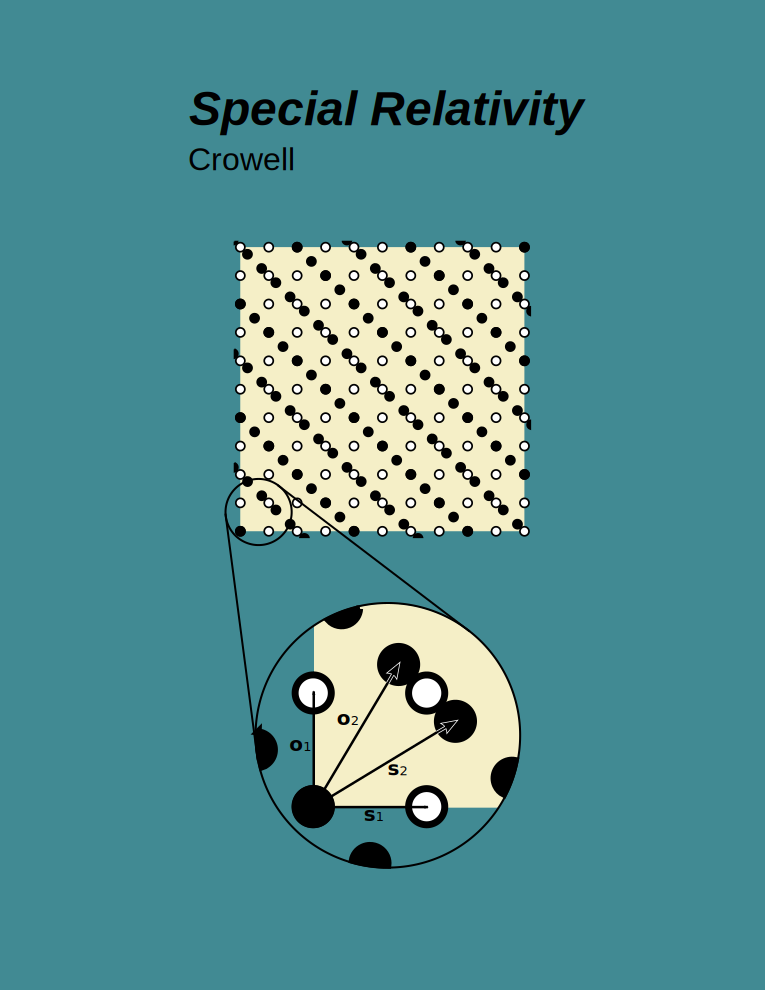
\includegraphics[width=\paperwidth]{cover/cover-for-pdf.png}\\
}
}%
\\


% ### COPYRIGHT ###############################################################

\renewcommand{\hintergrund}{images/seite.jpg}
\thispagestyle{empty}

\vspace{100mm}

\noindent
\includegraphics{cover/lmlogo}\\
Fullerton, California\\
www.lightandmatter.com

\vspace{20mm}
\noindent
Copyright \copyright  2013 Benjamin Crowell

\vspace{20mm}
\noindent
rev. \today{}

\vspace{6mm}
\noindent
Permission is granted to copy, distribute and/or modify this
document under the terms of the Creative Commons Attribution
Share-Alike License, which can be found at creativecommons.org. The license
applies to the entire text of this book, plus all the illustrations
that are by Benjamin Crowell. All the illustrations are by Benjamin
Crowell except as noted in the photo credits or in parentheses
in the caption of the figure.
This book can be downloaded free of charge
from www.lightandmatter.com in a variety of formats,
including editable formats.


% ### ANLEITUNG ###############################################################

\renewcommand{\hintergrund}{images/seite.jpg}
%========================================================================
% NIP'AJIN Autorenpaket v1.1, (C) Markus Leupold-Löwenthal
%========================================================================
% Dieses Werk untersteht folgender Lizenz:
% Namensnennung–Weitergabe unter gleichen Bedingungen 3.0 Österreich
% (CC BY-SA 3.0) http://creativecommons.org/licenses/by-sa/3.0/at/
%========================================================================

\banner{Anleitung zum Autorenpaket}{Anleitung}\zlabel{Anleitung}

\begin{center}\itshape
Dieser Abschnitt gibt ein paar Hilfestellungen, wie das \nipajin-Autorenpaket verwendet werden kann. Natürlich sollte dieser Abschnitt im finalen Dokument vom Autor entfernt werden ;)
\end{center}

\begin{multicols}{2}

\mysection{Einführung}

Hallo! Schön, dass du dieses Autorenpaket verwenden möchtest. Es ermöglicht dir, mit relativ wenig Aufwand ein komplettes Rollenspiel zu schreiben und bietet dir als Ausgangspunkt eine vollständige Dokumentstruktur inkl. Cover, Layout und Regelanhang, damit eigenständige Werke entstehen können, die du auch veröffentlichen darfst. Die folgenden Punkte gilt es dabei zu beachten:

\aufzaehlung{
\item Technische Details, wie man das Autorenpaket bedient, findest du in der README Datei.
\item Der hier enthaltene Dokumentaufbau ist nur als Vorschlag zu betrachten.
\item Beachte, dass das \nipajin~Logo nicht frei ist, d.\,h. dass du nur die textuelle Version \zitat{\nipajin} verwenden darfst. Ebenso ist das \ludusleonis-Logo (Münze), sowie das TRiAS Logo nicht frei, bitte verzichte auf eine Verwendung und beachte die korrekte Groß-/Kleinschreibung dieser Namen.
\item Die im Autorenpaket enthaltenen Bilder (Cover, Seitenhintergrund, Überschriftenbanner) sind frei, d.h. du darfst sie 1:1 verwenden, oder abwandeln.
\item Dieses Dokument unterliegt der CC BY-SA. Bitte informiere dich auf der Creative Commons Webseite genau, was es bedeutet, auf so einem Werk aufzubauen. Du musst nämlich diese Lizenz auf \emph{alles}, was du davon ableitest, wieder anwenden. Das gilt auch, wenn du nur Teile in andere Werke übernimmst, \zB~dir \zitat{nur das Layout abschaust}. Weiters musst du dein gesamtes entstehendes Werk unter die CC BY-SA stellen -- du kannst also nicht Teile (\zB~Bilder!) davon aussnehmen. 
\item Bedenke auch, dass die CC BY-SA die kommerzielle Nutzung deiner Inhalte durch andere erlaubt und du daher auch selbst die nötigen Rechte haben musst, alles, was du integrierst (\zB~Bilder oder Texte aus anderen Quellen) unter diese Lizenz stellen zu dürfen.
\item Die CC BY-SA sagt \uA~aus, dass du dich zur Ableitung vom Original bekennen musst. Am einfachsten ist das, wenn du den Kasten im Impresssum \zitat{Dieses Werk nutzt das freie NIP’AJIN-System~\ldots} drinnen lässt. Damit bin ich \zitat{in der von mir festgelegten Weise} genannt und es ist leicht ersichtlich, wo das Original her kommt.
\item Wenn du Änderungen am Regelwerk vornimmst, darfst du das natürlich tun, mach aber bitte deutlich, dass und wo du dich vom Original entfernst. Verwende in diesem Fall nicht mehr \zitat{NIP'AJIN} als Namen, sondern gib der Abwandlung einen neuen Namen. Alternativ und für den Leser einfacher ist vermutlich, wenn du Settingregeln im Szenarioteil anführst und den Anhang intakt lässt. 
}

\noindent\textbf{Du bist selbst dafür verantwortlich, dass dein abgeleitetes Werk mit der CC BY-SA verträglich ist!}

\mysection{Offene Punkte}

Dies ist eine erste Version des Autorenpakets, daher ist natürlich noch Luft nach oben. Noch nicht enthalten, aber (für irgendwann) geplant, sind \uA:

\aufzaehlung{
\item Symbole: Die RPGDings Schrift, die ich für \nipajin~und \trias~entworfen habe, muss ich erst gesondert unter eine offene Lizenz stellen.
\item NSC-Blöcke: Die erstmals in Kurai Jikan eingeführten, runden NSC-Statistik-Blöcke mit runden Ecken.
\item CMYK/Drucksupport: z.\,Z. produziert das Autorenpaket RGB-PDFs, die sich für Digitaldruckereien aber nicht für den Offsetdruck eignen. Da ich hier ein komplexeres Script-Geflecht zur Konvertierung habe, ist das nicht so leicht, das für Außenstehende leicht verständlich zu extrahieren. 
\item Portierung des Autorenpakets auf andere Systeme (Word/OpenOffice/LibreOffice, Scribus, \ldots). Hilfe erbeten!
}

\noindent
Ich lerne übrigens selbst gerne dazu. Wenn dir am \LaTeX-Code etwas auffällt, was man besser machen kann, lass' es mich wissen! 

\end{multicols}

\newpage

% ### PROLOG ##################################################################

\renewcommand{\hintergrund}{images/seite.jpg}
%========================================================================
% NIP'AJIN Autorenpaket v1.1, (C) Markus Leupold-Löwenthal
%========================================================================
% Dieses Werk untersteht folgender Lizenz:
% Namensnennung–Weitergabe unter gleichen Bedingungen 3.0 Österreich
% (CC BY-SA 3.0) http://creativecommons.org/licenses/by-sa/3.0/at/
%========================================================================

\banner{Prolog \zitat{Mein Szenario}}{Prolog}\zlabel{Prolog}

\begin{center}\vfill
Der Spielleiter sollte folgenden Text zu Beginn des Szenarios vorlesen oder austeilen:
\vfill\end{center}

\begin{multicols}{2}\itshape

Hier kommt der Prolog hin.

\lipsum[1-6]

\end{multicols}

\newpage

% ### SZENARIO #################################################################

\renewcommand{\hintergrund}{images/seite.jpg}
%========================================================================
% NIP'AJIN Autorenpaket v1.1, (C) Markus Leupold-Löwenthal
%========================================================================
% Dieses Werk untersteht folgender Lizenz:
% Namensnennung–Weitergabe unter gleichen Bedingungen 3.0 Österreich
% (CC BY-SA 3.0) http://creativecommons.org/licenses/by-sa/3.0/at/
%========================================================================

\begin{center}
\noindent\emph{Dieses Szenario benutzt das Rollenspielsystem \logonipajin~aus dem Anhang (\seite{Regeln}).} 
\end{center}

\banner{Spielleiterinformationen}{Spielleiterinformationen}

\begin{multicols}{2}

\noindent
Der hier vorgeschlagene Aufbau eines Szenarios hat sich bei mir bewährt, ist aber natürlich nur eine Empfehlung~\ldots

\mysection{Überblick}

Hier kommt eine kurze Einführung hin, worum es in dem Szenario geht. Es sollen keine Details verraten, sondern dem SL geholfen werden, den Inhalt als (nicht) leitenswert zu beurteilen.

\lipsum[1]

\mysection{Setting}\zlabel{Setting}

Hier erklärt das Szenario das Umfeld, in dem es sich bewegt. Allgemeine Geographie, Geschichte usw. sind hier gut aufgehoben. Alles, was ein SL über den Prolog hinaus wissen muss, kann hier hinein. \zitat{Charakterwissen} sollte jedoch großteils schon im Prolog (\seite{Prolog}) den Spielern nahegebracht worden sein. 

\lipsum[2-4]

\mysection{Setting-Regeln}\zlabel{SettingRegeln}

Wenn es besondere Regeln für dein Setting gibt (\zB~Wahnsinn-Regeln für ein Horrorabenteuer), sind die besser hier als im settingunabhängigen Regelanhang aufgehoben.

\lipsum[18] 

\mysection{Verlauf des Szenarios}

Hier passt der rote Faden des Szenarios gut hin, oder bei einem Sandbox-Abenteuer eben die Information, dass es den Faden nicht gibt.

\lipsum[5-9]
 
\mysection{Einstieg ins Szenario}

Wie werden die Charaktere mit dem Szenario zu Beginn konfrontiert und was sind die ersten, wahrscheinlichen Handlungsmöglichkeiten? 

\lipsum[10-11]

\mysection{Spieltechnisches}

Einzelne Ortbeschreibungen, NSCs, Monster und Spielwerte passen hier gut hin, wenn sie über allgemeine Informationen vom Abschnitt \zitat{Setting} (\seite{Setting}) hinaus gehen.

\lipsum[12-15]

\mysection{Ende gut, alles gut?}

Mögliche Enden des Szenarios oder ein Epilog, soweit vorhanden, gehören hier hin. Zudem passt hier noch gut ein Ausblick hin, wie ein SL das Szenario bei Gefallen selbst weiter gestalten könnte.

\lipsum[16-17]

\end{multicols}

\newpage

% ### REGELN ###################################################################

\renewcommand{\hintergrund}{images/seite.jpg}
%========================================================================
% NIP'AJIN Autorenpaket v1.1, (C) Markus Leupold-Löwenthal
%========================================================================
% Dieses Werk untersteht folgender Lizenz:
% Namensnennung–Weitergabe unter gleichen Bedingungen 3.0 Österreich
% (CC BY-SA 3.0) http://creativecommons.org/licenses/by-sa/3.0/at/
%========================================================================

\hyphenation{Mana}
\hyphenation{LUDUS}
\hyphenation{LEONIS}

\noindent
\begin{center}
\emph{Im folgenden Anhang findet sich das vollständige \logonipajin~Regelwerk (Version~v1.3).}
\end{center}

\banner{Anhang I -- Regeln für Spieler}{Regeln für Spieler}

\begin{multicols}{2}

\mysection{Was ist \nipajin?}\zlabel{Einleitung}\zlabel{Regeln}

\nipajin, ein unkompliziertes, universelles Rollenspielsystem von \ludusleonis\ für Einzelabenteuer und Kurzkampagnen, ist ein Akronym für \zitat{Niemand ist perfekt, aber jeder irgendwie nützlich} und wird \zitat{nip-ah-tschin} ausgesprochen. Es sorgt für verteiltes Rampenlicht zwischen den Charakteren, ohne diese in ein enges Regelkorsett zu zwingen. Eine Erklärung, was ein Rollenspiel ist, würde hier den Rahmen sprengen -- bei Bedarf kann das auf \href{http://www.ludus-leonis.com/}{http://www.ludus-leonis.com/} nachgelesen werden.

\mysection{Erschaffung}\zlabel{Erschaffung}

Jeder \wichtig{Charakter} startet als unbeschriebenes A4-Blatt im Querformat. Dieses \wichtig{Charakterblatt} wird durch eine Linie in zwei A5-Hälften geteilt, dann die rechte Hälfte in zwei A6-Viertel geteilt. 

Nun kritzeln die Spieler allgemeine Charakteristika wie Name, Volk und Aussehen in die linke Hälfte, gefolgt vom \wichtig{Hintergrund} des Charakters. Dies kann in Stichworten oder Prosa geschehen. Die Beschreibung enthält, was ein Charakter bisher gemacht hat, und nicht, was er gut kann. Letzteres wird der Spielleiter erst im Spiel anhand des Hintergrunds entscheiden. Am Charakterblatt steht dann \zB\ \zitat{war jahrelang Klavierträger} statt \zitat{ist stark}. Die \wichtig{Ausrüstung} (\seite{Ausruestung}) und die beherrschten \wichtig{Effekte} (\seite{Magie}) enthalten, was Spieler und Spielleiter für richtig befinden. 

Zuletzt werden je ein W4, W6, W8, W10 und W12 auf das rechte obere Viertel gelegt. Einer dieser fünf Würfel wird vom Spieler zum \wichtig{Widerstandswürfel} \WW\ ernannt und mit der Eins nach oben in die linke Blatthälfte gelegt. Überschreitet er später im Spiel seine Kapazität (\zB\ eine Sieben am W6), scheidet der Charakter aus.

\mysection{Würfelsystem}\zlabel{Wuerfelsystem}

Solange es keine Zweifel gibt, blubbert die Handlung zwischen Spielern und Spielleiter fröhlich vor sich hin. Stellt sich aber bei einer handlungsrelevanten \wichtig{Aktion} die Frage, ob sie einem Charakter gelingt, wählt sein Spieler einen \wichtig{verfügbaren Würfel} aus dem oberen Viertel des Charakterblatts und würfelt. Fällt eine Eins, ist die Aktion ein \wichtig{automatischer Fehlschlag}. Ansonsten wird ein, von der \wichtig{Expertise} des Charakters abhängiger \wichtig{Modifikator} zum Wurf addiert, den der Spielleiter anhand des Charakterhintergrunds festlegt.

\tabelle{X c}{
\thead{Expertise} & \thead{Modifik.} \\
}{
veritable Schwäche                   & -4 \\
unerfahren, sehr ungeschickt         & -2 \\
etwas eingerostet                    & -1 \\
durchschnittlich gut                 &  0 \\
ein wenig Übung, Hobby               & +1 \\
jahrelange Erfahrung, Beruf, Routine & +2 \\
jahrzehntelange Erfahrung, Veteran   & +4 \\
}

\noindent
Erreicht oder übertrifft der resultierende \wichtig{Endwert} den vom Spielleiter vorgegebenen \wichtig{Zielwert}~\ziel\ der Aktion, gelingt diese. Ein Endwert von Eins ist im Gegensatz zur gewürfelten Eins kein automatischer Fehlschlag, aber selten hoch genug.

Nach dem Wurf wird der nun \wichtig{verbrauchte Würfel} in das untere Viertel des Charakterblatts gelegt. Erst wenn \emph{alle} Würfel verbraucht sind -- und nur dann! -- kann ein Spieler seinen Charakter \wichtig{durchatmen} lassen, ehe die Würfel wieder nach oben gelegt werden: Er muss kurz -- während eines Konflikts eine komplette Runde -- aussetzen.

\tabelle{l c X}{
\thead{Schwierigkeit} & \thead{\ziel} & \thead{Beispiel} \\
}{
einfach               & 2 & -- \\
gute Bedingungen      & 3 & gutes Werkzeug \\
durchschnittlich      & 4 & -- \\
schlechte Bedingungen & 5 & wenig Licht \\
schwer                & 6 & Messer jonglieren \\
meisterlich           & 8 & Drahtseilakt \\
legendär              & 10 & -- \\
}

\noindent
Wurde für einen Wurf ein neuer Modifikator festgelegt, sollte der Wert auf dem Charakterblatt notiert werden, damit er nicht mehrfach bestimmt werden muss. Würfel ohne Chance auf einen Erfolg dürfen nicht geworfen bzw. verbraucht werden. 

Bei einem \wichtig{Gruppenwurf} versuchen Charaktere gemeinsam, einen -- oft sehr hohen -- Zielwert zu erreichen. Die beteiligten Spieler wählen zeitgleich je einen Würfel, aber nur der größte wird vorerst benutzt (\zB\ W8 vor W6). Der würfelnde Spieler entscheidet, ob der erreichte Endwert als Gruppenergebnis genügt. Wenn nicht, darf der Spieler mit dem nächstgrößeren Würfel versuchen, das Gruppenergebnis zu erhöhen, usw. Ein automatischer Fehlschlag vereitelt den Gruppenwurf. Nur die tatsächlich benutzten Würfel werden verbraucht.

Beim \wichtig{Nachbessern} kann ein zu schlechter Wurf eines Spielers von einem anderen wiederholt werden, wenn die Handlung das zulässt. Der Zielwert erhöht sich dabei um 1. Jeder Charakter darf ein Mal nachbessern, der Zielwert erhöht sich dabei kumulativ. 

\mysection{Konflikte}\zlabel{Konflikte}

Interessenskonflikte werden in \wichtig{Runden} abgehalten, deren Länge der Spielleiter festlegt. Jede Runde darf jeder Charakter eine Aktion durchführen, \zB\ angreifen, und auf alle Aktionen seiner Gegner reagieren, \zB\ parieren. Die \WW\ der Gegner sind zu überwinden, egal ob mit oder ohne Gewalt.

Zu Beginn jeder Runde wählen alle Spieler zeitgleich je einen \wichtig{Aktionswürfel} \AW\ und einen \wichtig{Reaktionswürfel} \RW\ aus ihren verfügbaren Würfeln. Mit diesen bestreiten sie diese Runde alle Aktionen bzw. Reaktionen. Freiwillig, oder wenn zu wenig Würfel verfügbar sind, kann auf den \AW\ oder \RW\ und damit auf Aktionen bzw. Reaktionen verzichtet werden. Wer \emph{keine} verfügbaren Würfel mehr hat, darf durchatmen.

Der gewählte \AW\ gibt auch die \wichtig{Initiative} in der Runde an. Kleine Würfel handeln vor großen (\zB\ W6 vor W8). Bei Gleichstand würfeln die Betroffenen die Initiative aus.

Für einen erfolgreichen Angriff muss der \AW\ einen höheren Endwert aufweisen als der \RW, eine \emph{gewürfelte} Eins ist immer ein Fehlschlag. Bei einem erfolgreichen Angriff erleidet der Reagierende eine \wichtig{Wunde} und zählt diese am \WW\ hoch. Auch gewaltlose Aktionen helfen, den Widerstand der Gegner zu brechen: Sie verursachen \wichtig{Traumata}, die durch Spielsteine symbolisiert oder auf einem extra W20 gezählt werden. Überschreitet die Summe aus Traumata und aktuellem \WW-Stand den \WW, ist der Gegner überwunden (eingeschüchtert, irritiert,~\ldots). 

Charaktere können auch im Konflikt einen Gruppenwurf gegen \emph{einen} Gegner versuchen. Es gilt die Initiative des schlechtesten Gruppenmitglieds, dafür tritt der Gegner mit seinem \RW\ gegen das Ergebnis an. Es droht die Summe der Wunden der einzelnen Würfe.

Ein Charakter kann via \wichtig{Flächenangriff} mehrere Gegner angreifen (\zB\ Rundumschlag, Gruppen einschüchtern, Feuerball,~\ldots). Pro zusätzlichem Ziel wird der Wurf um -2 modifiziert. Jeder Gegner darf individuell reagieren.

Letztlich kann ein Charakter andere \wichtig{decken}, wenn er diese Runde keinen \AW\ wählt. Er darf dafür die Angriffe von Gegnern in Reichweite im Ausmaß seines halben \RW\ auf sich umleiten, \zB\ zwei beim W4 oder drei beim W6. Misslingt dem Deckenden eine solche Reaktion, bekommt er selbst die Wunden.

\mysection{Heilung}\zlabel{Heilung}

Nach jeder \wichtig{Nachtruhe} wird durchgeatmet. Zudem kann versucht werden, die Wunden am \WW\ zu verringern. Der Spieler merkt sich den Wert und würfelt den \WW. Wird der Wert unterwürfelt, verheilt eine Wunde. Der \WW\ wird in diesem Fall um eins niedriger wieder hingelegt, sonst mit dem ursprünglichen Wert.

\wichtig{Traumata} verheilen abhängig von ihrem Ursprung nach Maßgabe des Spielleiters. Einschüchterungsversuche klingen schon am Ende der jeweiligen Szene wieder ab, Ängste, Flüche, etc. schleppen die Charaktere manchmal tage- oder wochenlang mit.

\mysection{Ausrüstung}\zlabel{Ausruestung}

Es gibt keine Ausrüstungstabelle. Normale Waffen verursachen grundsätzlich eine Wunde pro Treffer, besondere oder magische Waffen zwei und Feuer- oder Explosivwaffen drei bis vier. Improvisierte Ausrüstung bedingt -1 auf den \AW. Rüstungen geben je nach Ausführung +1 oder +2 auf den \RW.

\end{multicols}

\banner{Anhang II -- Regeln für Spielleiter}{Regeln für Spielleiter}

\begin{multicols}{2}

\mysection{Effekte}\zlabel{Magie}

Von Charakteren beherrschte Magie, Wunder, PSI-Kräfte, Superkräfte u.ä. werden \wichtig{Effekte} genannt und bereits bei der Erschaffung festgelegt. Sie sind, so überhaupt im Szenario erlaubt, auch dort geregelt, berufen sich aber u.\,U. auf folgendes \nipajin-Standardsystem:

Eine \wichtig{Vorbereitungszeit} \VZ\ lang murmelt oder gestikuliert der Wirkende. Ist sie \wichtig{variabel}, wird sie nach Bedarf vom Spieler festgelegt. Es folgt der Wurf, ggf. mit den üblichen -2 pro Zusatzziel bei Flächenangriffen. Dem Opfer steht ein Reaktionswurf zu, um dem Effekt vollständig zu entgehen. Gegenstände und opferlose Effekte haben einen vom Spielleiter festgelegten Zielwert. Bei Gelingen hält der Effekt an, solange sich der Wirkende konzentriert, zzgl. einer \wichtig{Nachwirkzeit} \NWZ. 

\wichtig{Nahkampfeffekte} verwunden wie Nah\-kampf\-waf\-fen, \zB\ \emph{Frosthand} oder \emph{Geisterschwert}. Ein Treffer verursacht eine Wunde. \VZ:~1~Runde; \NWZ:~$\infty$

\wichtig{Fernkampfeffekte} verwunden wie Fern\-kampf\-waf\-fen und verbrauchen pro Anwendung eine limitierte Ressource, \zB\ benötigt \emph{Magisches Geschoß} Pulver aus dem Gürtelbeutel, \emph{Feuerball} eine Art magische Handgranate. \VZ:~1~Runde; \NWZ:~$\infty$

\wichtig{K.\,O.-Effekte} machen Wesen handlungsunfähig, \zB\ \emph{Schlaf}, \emph{Versteinerung}, \emph{Angst} oder \emph{Bannen}. \VZ:~variabel; \NWZ:~aufgewandte \VZ

\wichtig{Unterstützungen} helfen einem Wesen oder verbessern einen Gegenstand in einem Aspekt, \zB\ \emph{Feuerresistenz}, \emph{Federfall}, \emph{Barriere} oder \emph{Licht}. \VZ:~variabel; \NWZ:~aufgewandte \VZ

\wichtig{Veränderungen} verformen oder bewegen langsam tote Materie bzw. Gefühle von Wesen, \zB\ \emph{Wasser-zu-Wein}, \emph{Befreunden} oder \emph{Telekinese}. \VZ:~variabel; \NWZ:~aufgewandte \VZ

\wichtig{Illusionen} täuschen einen Sinn eines Wesens für ein konkretes Detail, \zB\ \emph{Katzengold}, \emph{Täuschgeräusch} oder \emph{Unsichtbarkeit}. \VZ:~variabel; \NWZ:~aufgewandte \VZ

\wichtig{Eingebungen} verschaffen Wissen über Eigenschaften oder Sachverhalte, \zB\ \emph{Magie spüren}, \emph{Gedanken lesen} oder \emph{Hellsicht}. \VZ:~eine Minute für Gegenwärtiges, eine Stunde für Vergangenes, ein Tag für Zukünftiges; \NWZ:~--

\wichtig{Heileffekte} schließen Wunden oder heilen Krankheiten. \VZ:~eine Stunde pro Wunde, ein Tag pro Krankheit; \NWZ:~$\infty$

\mysection{Spielercharaktere}\zlabel{Spielercharaktere}

Den Hintergrundbeschreibungen der Spielercharaktere (SC) kommt in \nipajin\ besondere Bedeutung zu. Gute Hintergründe umschreiben Kindheit, Ausbildung und was der SC in den letzten Jahren hauptsächlich getan hat. Ein paar einschneidende Erlebnisse runden das Bild ab. Auch Alter und Aussehen eines SC sollten festgehalten werden. 

Es liegt am jeweiligen Spielstil, wie formell ein Hintergrund ausfallen muss. Der Spielleiter sollte darauf achten, dass er genügend Rückschlüsse auf die Stärken und Schwächen des SC ermöglicht, da im Zweifel auf dieser Basis entschieden wird, ob eine Aktion leicht- oder schwerfällt. Lücken im Hintergrund sollten im Einverständnis mit dem Spieler sofort geschlossen werden.

\mysection{NSCs}\zlabel{Nichtspielercharaktere}

Der Spielleiter wird den SC eine Reihe von Freunden und Feinden entgegensenden. Bei deren Gestaltung stehen zwei Wege offen.

\wichtig{Zentrale Nichtspielercharaktere} (NSC) einer Geschichte können, wie die Charaktere auch, mit einem definierenden Hintergrund ausgestattet werden, der Stärken und Schwächen enthält. Dies sollte aber nicht übertrieben werden, eine gute Geschichte benötigt selten mehr als ein, zwei solcher NSC. Treten die SC gegen sie an, behandelt der Spielleiter seine NSC als gleichwertig und verwendet die Regeln aus dem Spielerteil. 

Das \zitat{Gros} der NSC hat nur eine \wichtig{Nebenrolle}. Sei es der Informant, der Händler am Basar oder das lästige Monster von nebenan. Um den Spielleiter vor und im Spiel zu entlasten, werden diese Figuren vereinfacht geregelt. Neben dem Aussehen und der Motivation, mit den SC zu interagieren, genügt es, pauschal den \WW, \emph{einen} \AW\ und \emph{einen} \RW\ festzulegen. Daneben werden paar Stichwörter zu Stärken und Schwächen notieren. Als \WW\ ist alles von 1 bis $\infty$ erlaubt, als \AW/\RW\ das Würfel-Set aus W2, W3, W4, W5, W6, W8, W10, W12 und W20. Traumata werden direkt am \WW\ und nicht extra gezählt. Nebenrollen haben gegenüber SC den Vorteil, nicht durchatmen zu müssen, da ihnen die \AW/\RW\ nie ausgehen. Sie sollten zum Ausgleich etwas unterdimensioniert werden. % Beispiele finden sich im~\ldots

\mysection{Erfahrung}\zlabel{Erfahrung}

Jeder Charakter erhält pro Sitzung einen \wichtig{Charakterpunkt} (CP). Eine Expertise um Eins zu verbessern kostet so viel, wie der neue Wert betragen soll; eine Schwäche um Eins zu mildern dagegen so viel, wie der alte Wert beträgt (+2 auf +3 = 3 CP, -2 auf -1 = 2 CP).

In \nipajin\ definieren die SC das Niveau der Welt. Verkörpern sie durchschnittliche Abenteurer, sind die im Bestiarium angegebenen Beispiele gute Richtwerte für \zitat{die Anderen}. Verkörpern sie jedoch \zB\ selbst Goblins, die sich Scharen von \zitat{Helden} erwehren müssen, die über ihr Lager herfallen, sind die Charaktere für diese \zitat{Helden} vielleicht nur Goblins, aber für die Goblins ist ein \zitat{Held} vielleicht schon mächtig wie ein Troll. Der Spielleiter sollte die Werte von SC und NSC nur relativ zueinander betrachten.

Sollten die SC über Nacht an Super\-hel\-den\-kräfte gelangen, empfiehlt es sich, \emph{nicht die Charaktere} zu steigern, \emph{sondern die Welt} um sie herum entsprechend abzusenken!

\mysection{Bestiarium}\zlabel{Bestiarium}

Die folgenden Kreaturen dienen nur der Veranschaulichung und sollen \nipajin\ nicht auf bestimmte Hintergründe festlegen. 

\tabelle{p{1.2cm} c c c X}{
\thead{Kreatur} & \thead{W} & \thead{A} & \thead{R} & \thead{Fähigkeiten}  \\
}{
gr. Ratte & 1 & 2 & 3 & Laufen+4, Verstecken+2 \\
Goblin & 3 & 4 & 4 & Wahrnehmung+1 \\
Ork & 6 & 6 & 6 & Einschüchtern+1, Kämpfen+1, Verstand-1 \\
Troll & 10 & 8 & 6 & Kämpfen+2, regeneriert eine Wunde/Runde \\
Riese & 20 & 8 & 8 & Kämpfen+2, Kraft+4 \\
Drache & 40 & 12 & 10 & Feueratem+4, K.\,O.-Effekt-Resistenz \\
}

\end{multicols}

\vfill

\banner{Anhang III -- Beispielcharaktere}{Beispielcharaktere}

\vspace*{1em}

{\noindent \centering \emph{Die folgenden Seiten enthalten schlüsselfertige Charaktere, mit denen sofort losgespielt werden kann.}

} 


% ### CHARAKTERE ###################################################################

\renewcommand{\hintergrund}{images/characterblatt.jpg}
%========================================================================
% NIP'AJIN Autorenpaket v1.1, (C) Markus Leupold-Löwenthal
%========================================================================
% Dieses Werk untersteht folgender Lizenz:
% Namensnennung–Weitergabe unter gleichen Bedingungen 3.0 Österreich
% (CC BY-SA 3.0) http://creativecommons.org/licenses/by-sa/3.0/at/
%========================================================================


% ###############################################################
\charakter{

\mysection{Charakter No.\,1}

\lipsum[1]

\subsection*{Eigenschaften}

Größe, Aussehen, usw. 

\vspace{1em}

Spielwerte: \emph{Dieses+1, Jenes-2}

}

% ###############################################################
\charakter{

\mysection{Charakter No.\,2}

\lipsum[2]

\subsection*{Eigenschaften}

Größe, Aussehen, usw. 

\vspace{1em}

Spielwerte: \emph{Dieses-1, Jenes-2, DafürDasDa+3}

}


% ### BACKCOVER ################################################################

\renewcommand{\hintergrund}{images/backcover.jpg}
\thispagestyle{empty}
\pagecolor{coverbackground}\afterpage{\nopagecolor}

\corner{63}
\centering

\begin{center}
	{\Large \textbf{LIKE A BOSS} \par}
	\vspace{0.3cm}
	\pgfornament[width=5cm]{84}
	\vspace{0.5cm}
	{\par J'ai entrepris l'écriture de ce livre car je n’ai pas trouvé d’ouvrages s’adressant aux jeunes ambitieux désirant réussir professionnellement. Pourtant, des millions d’étudiants passent par cette étape de la vie tous les ans.}
	\vspace{0.2cm}
	{\par Je te souhaite donc une très bonne lecture en espérant lire tes critiques par email ou sur Twitter.}
	\vspace{0.5cm}
	{\par \textbf{AZIKA-EROS} Christ Michel}
	{\par christ @ azika-eros.org}
	{\par twitter.com/supm4n \\}
	{\par http://christ.azika-eros.org \\}
	\vspace{0.5cm}
	\pgfornament[width=2cm,symmetry=h]{69}

\end{center} 

\end{document}
